\documentclass[11pt,a4paper]{report}

\usepackage[utf8]{inputenc}
\usepackage{amsmath}
\usepackage{natbib}
\usepackage{url}
\usepackage{listings}
\usepackage{graphicx, wrapfig}
\usepackage[font=small,labelfont=bf]{caption}
\usepackage{float}
\usepackage{afterpage}
\usepackage{appendix}
\usepackage{minted}
%\usepackage{hyperref}
%Fancy Header-----
\usepackage{fancyhdr}
\setlength{\headheight}{14pt}%
\pagestyle{fancy}
\fancyfoot{}
\renewcommand{\footrulewidth}{0.0pt}
\renewcommand{\headrulewidth}{0.0pt}
\lhead{CMP3060M - Project - 
Assessment Item 2 - Project Report}
\rhead{}
\fancyfoot[R]{\thepage}
\fancyfoot[L]{PRO14514822 - Owen Prosser}
\fancypagestyle{plain}{\pagestyle{fancy}}
%-------------
%Fancy Header-----
\usepackage{afterpage}
\newcommand\blankpage{%
    \null
    \thispagestyle{empty}%
    \addtocounter{page}{-1}%
    \newpage}
\graphicspath{ {images/} }
%-------------

%Harvard Referencing
\bibliographystyle{agsm}

%Setup the title
\title{
	{AN INVESTIGATION INTO THE DEVELOPMENT AND EFFECTIVNESS OF COMPUTER-VISON FALL DETECTION SYSTEMS AT THE UNIVERSITY OF LINCOLN}\\
	{\large University Of Lincoln}
}
\author{PRO14514822 - Owen Prosser}
\begin{document}
%Insert the title
\maketitle

\begin{abstract}
\emph{The overall aim of this project is to create a Fall Detection System using the Python programming language and its OpenCV library. This system is intended for to assist families, or care-providing professionals, who are responsible for the well-being of the elderly but cannot for whatever reason monitor them at all times. It is designed to alert any kind of care-giver in the event of an elderly person having had a fall with the possibility of hurting themselves potentially requiring medical attention, or, just some reassurance and compassion.}
\end{abstract}

%\afterpage{\blankpage}

\tableofcontents
\pagebreak
\listoffigures

%\afterpage{\blankpage}

\chapter{Literature Review}
\section{Background}
According to the World Health Organisation a fall is the second leading cause of ``unintentional injury deaths" worldwide, making this an issue of the highest severity \citep{Cruz_Fall_detection_wearable_device}. The population is aging in most western countries. In the US, in the 28 years from 1980 from 2008, the share of the population over 60 has nearly doubled from 9.9 million to 18.6 million \citep{Siracuse_Health_care_and_socioeconomic}. 30\% of both independent and institutionalised persons over the age of 75 are estimated to experience a traumatic fall in a year \citep{Sixsmith_A_smart_sensor_to_detect}, thus putting the elderly at a significantly higher risk of ``injury to the head, neck, and pelvis than younger individuals"  These falls a huge issue for the elderly population as it is estimated that 90\% of geriatric injuries are caused by falls \citep{boltz_Injuries_and_outcomes}. This puts a huge strain on hospitals as well as families who care for elderly relatives. A system for detecting these falls should they occur could assist carers for the elderly as they would not have to be with the cared at all times. This would both reduce the workload for the carer and give back some privacy and independence. It has also been shown that ``longer the lie on the floor, the poorer is the outcome of the medical intervention"\citep{Li_A_microphone_array}. A detection system which could alert a care giver quickly could reduce the delay between the fall and provision of medical assistance increasing the chances of a good recovery and lowering distress for the patient.

\section{Available Systems}
There are many currently available alarm systems for detecting human falls. These are generally split into two categories; user-activated systems where the user manually actives an alarm after a fall, and automatic systems where the alarm is triggered without user interaction once a fall is detected \citep{Alwan_A_smart_and_passive_floor-vibration}. 

\section{Wearable Systems}
A large portion of these automatic systems require the user to wear specialised equipment or carry a specialised device with them at all times. These devices are then used to track the motion and/or location of the user. One of these type of systems uses the accelerometer, which is built into most modern smart phones, to detect falls \citep{Tsinganos_A_smartphone-based_fall}. This works by sensing a sudden change in acceleration of the device. This system has a precision of 91.8\% making it fairly accurate but also has a some fundamental drawbacks. Firstly, the system's accuracy is affected by how the user is carrying their phone and where it is placed on their body (if it is in a pocket or being held) and of course it will have an accuracy of  0\% when the phone is not being carried or is not running the app. 

Many systems attach specialised hardware to the body of the user(using wearable devices or by integrating them into clothing) to measure their acceleration to detect falls. One of these systems uses a `pendant' worn around the user's neck \citep{Santiago_Fall_detection_system}. The detection system works in a similar way to the previous smartphone-app-based system, this time with the pendant containing dedicated hardware to measure changes in acceleration rather than using the multi-purpose sensors built into the users smartphone. This pendant then communicates with a smartphone app to trigger an alert if a fall is detected. This system has a very similar accuracy to the afore mentioned smartphone-based system rate of 92\% but has the advantage that this should be more consistent as the detector will always be placed in the optimised area of the user's body when compared to a smartphone which will be moved. Another system utilises a custom sensor unit attached to the belt of the user \citep{Cruz_Fall_detection_wearable_device}. Whilst the accuracy of the system is not present in this paper, it is safe to assume that it would be similar to that of the previous system as they both feature a similar hardware implementation and methodology for establishing the acceleration threshold to determine a fall. Without evidence of a significant improvement in the quality of detection, this system appear to be less practical than the previous system as the belted sensor array is bulkier and probably less comfortable to wear. 

Systems which rely on wearable hardware have been described as an ``unfavourable choice for the elderly" \citep{fallDetectionInvestigation}. These systems still require that the user wear a specialised piece of hardware at all times to function. Although this is better than having to carry a smartphone this is still not ideal for elderly users. One severe limitation of all smartphone-based systems is that they require the user to already own a smartphone. This is a limiting factor because whilst smartphone adoption is on the rise among the over 55 age group only 30\% of this category currently own a smartphone \citep{Berenguer_Are_Smartphones_Ubiquitous}. The potential user base for a fall detection system could be greatly expanded if the system was functional on its own, without being reliant, for example, on the user's smartphone connection to the Internet to trigger and alarm in the event of a fall as many elderly people ``are having difficulties in using modern smart devices" \citep{William_Cognitive_modeling_in_human_computer_interaction}. A system which does not require the direct interaction of the user to function could be more effective at detecting falls as it can be passively running in the background; in no way reliant on input from the user, or their aptitude for technology.

\section{Passive Systems}
Passive systems use a variety of sensing methods to detect falls, including: cameras, Infra-Red (IR) thermal-imaging cameras or ultra-sonic sensors. One of the most effective of these systems uses ultrasonic sensors to detect the area of the floor of a room which is covered by the user. When walking around the house normally the user's feet will only cover a small section of the floor space, in the event of a fall, the user's body will cover a larger area of the floor, the system will detect this as a fall \citep{Chang_Human_fall_detection_based_on_event}. This system is very accurate with ``up to 98\% precision" but it does require a large amount of hardware, which has to be installed around the perimeter of each room where fall detection is required. 

Another passive system uses a ceiling-mounted IR camera to gather a top down heat-map of the room. \citep{Hayashida_The_use_of_thermal_ir_array}. When the user is moving around the monitored space normally, the camera will perceive a small area being at a higher temperature than the rest of the room. If the user is to fall over in view of the thermal-camera their thermal signature will appear larger to system, allowing it to detect a fall. This system is effective at its goal of detecting falls with a ``robust fall recognition rate of over 94\%" but requires specialised thermal imaging hardware. This hardware, at its current cost, would be prohibitively expensive not only to this project but also to the system's end user. 

One other passive system utilises a circular array of 8 omni-directional microphones to detect a fall based on the noise of the users body's contact with the floor \citep{Li_A_microphone_array}. The main drawback of this type of system is that its accuracy is somewhat dependent on the acoustic conditions of the room. Any background noise from traffic or a television can mask the sound of a fall potentially allowing for it to be missed. This shortcoming is not shared by systems which rely on cameras (including thermal imaging cameras) as these are not as easily affected by interference.

\section{Detecting Falls}
The Passive Fall-Detection systems detect when the user has fallen using a number of different methods and algorithms. One system uses the angle of the Major and Minor axes of an ``approximate ellipse" around the silhouette of the user \citep{rougier2007fall}. This is shown to work effectively as the referenced system was tested with 17 falls and correctly detected 15 of them \citep{rougier2007fall}. This solution is also relatively understandable and could potentially contribute to a straight-forward implementation as it requires no additional or specialised hardware. Some of the other passive systems require hardware other than a standard web cam to operate. For example one passive system uses the RGB-D (Red, Green, Blue and Depth) sensor built into the Microsoft Kinect depth sensing system \citep{kinectPassiveDetection}. Another visual camera-based system uses ceiling-mounted, overhead image sensors\citep{nait2004activity}. This detection method works by ``shape change analysis as well as inactivity detection" from an overhead view \citep{fallDetectionInvestigation}.

\section{Conclusions}
Many elements of the discussed research is relevant and will have an affect on this project. Firstly, it is important that the system is active at all times as a fall can be severely damaging to the health and well-being of an elderly person. Consequently the Fall Detection System should not be configured or operated by the monitored-person as they are likely to be elderly and thus not particularly technologically literate.

The user would also benefit from any specialised wearable-hardware not being a requirement for the operation of the system. This would allow the user a fuller freedom of movement and more comfort in their home.


This Passive system will also function using a method similar to that of \cite{rougier2007fall}. This is due to certain limitations of this project. In this project it is not feasible to acquire and use non-standard hardware as mention in Section 1.5 for reasons of both cost, and the time restrictions placed on the project. As it would take significant effort to configure and develop such a system.

\chapter{Methodology}

\section{Project Management}
This project was developed using an agile methodology. The development of the artefact was divided into many one week long iterations each beginning/concluding with a meeting with the project supervisor. Each of these meetings began with a brief discussion of the progress made during the previous week. This part of the meeting was then followed by a discussion of the tasks to be undertaken before the next meeting. This follows the structure of an iterative methodology.

An iterative methodology also focuses on breaking down the entire project into small parts, each of these parts is then set to be completed during one of the many iterations. At the beginning of the development process the requirements of the project are analysed to find how they can best be divided into their component parts for each of the development iterations. The most important factor during this part of the process is that this set of requirements is well defined. This allows for the project to be accurately divided, without having to repeat this part of the process again if and when the requirements become more clearly defined. This was useful during this project as the requirements were very well-defined from the beginning of the project and have not changed during its development. The progress of the project is made easier to track when it is divided into many parts in this way. Throughout the entire project it is known how many parts are left to complete and what is required to complete each of them. The progress can also be precisely known because the project is being undertaken by an individual, rather than a team. This means that it is not required to understand how other members of the team are working and what progress they are making with the development.

Another of the main purposes of using an iterative methodology is to allow the individual to be more adaptable if, and when, an obstacle to the development process does arise \citep{Wiley_Project_Management}. After a break in productivity due to a change in the system's requirements or other unforeseen circumstance, an iterative project management methodology can adapt to this change. This is due to the structure of the methodology, with many regular meetings, each with its own set of goals. These meetings allow for a team, or individual developer, to realign and reorder the upcoming tasks based on the best-known way to navigate this new landscape of requirements. One example of where this was used during the completion of this artefact was that there were many other unrelated tasks which needed to be completed in parallel with this project. This had the affect of causing some delays throughout the development process, as these other tasks could often have their own delays and unforeseen changes. 

This kind of individual sprint is only possible with a small scale development such as this, usually an individual would not be able to focus themselves in one particular area for an extended period of time without it being detrimental to their other responsibilities, for example, if they were trying to run a small independent business they would have other tasks to complete other than software development. 

However, this approach can have some drawbacks in terms of a project such as this. As this is a small project undertaken by an individual without much oversight, there is the possibility of getting lost and not making sufficient progress towards the overall goal caused by constantly changing direction with each iteration of the development.

An iterative Agile methodology is advantageous over a non-agile methodology like Waterfall. When using Waterfall, for example, each stage of development has to be completed before the next can begin. This can cause large delays when one part of the project is experiencing delays. This would be particularly problematic for a project such as this as delays can be common for all parts of this development for many reasons. Firstly, many other unrelated tasks were also required their own dedicated time to complete during the development of the artefact. This would have caused long delays under the Waterfall development method as it would have prevented development on any other part of the artefact until these other tasks had been fully completed. Also as some time was required to be spent researching and learning how to use some of the vital components of this project (such as OpenCV), this would have caused other parts of the development to completely stall under the older, non-agile Waterfall methodology. 

\pagebreak

\section{Software Development}
When creating any piece of software in a confined time scale it is important that there is some system in place to ensure the software is being written in an efficient manner. In order to do this effectively, it has to be managed within the limitations of the project at hand. This project has many factors which impact the available software engineering methodologies that could be effectively employed to increase the speed of development and improve the quality of the artefact in relation to its original aim and objectives. The main factors which affected how the development of the project was carried out were, firstly, this was a project for one individual to complete, it had a very strict deadline for completion, which could not be extended. There were many other unrelated tasks which needed to be completed in parallel. In addition to these factors there were many unfamiliar components to be used for the development of the system which required specific time set aside for them to be researched, for both there operations and implementations.

This project did however have one quality to the benefit of various Software Engineering Methodologies; the project had very well defined requirements from the beginning, this can be vital during the planning stages, which are an important part of many methodologies.

The oldest, and still one of the most commonly used development methodologies, is the Waterfall methodology \citep{shaydulin2017agile}. This methodology was not used for a number of reasons. Firstly, as the time to complete this project was limited, the Waterfall methodology could have contributed to incorrectly allocating time to certain areas of the project where it was not as valuable as in others. This would have been due to the strictly linear nature of the methodology, dictating that some parts of the project (such as requirement gathering and analysis) had to be completed before other stages could begin \citep{shaydulin2017agile}. This would have been an issue for this project as it carried out by an individual with other, also important, concerns during the development period. Without being able to switch between the different tasks and areas of the project as the available time permitted within a busy schedule, the development could have stagnated. 

The Waterfall methodology has a rigid structure which does not allow the developer(s) to repeat a stage without completing all subsequent stages until the end of the cycle \citep{WaterfallPresentation}. This would not allow for the software to be thoroughly tested during the development process as this would have had to have been added as an additional stage at the end of the Waterfall cycle. This would have been detrimental to the development of the artefact because it relied on testing throughout the development to ensure that it was functioning correctly, and any new features that had been added since the last set of tests had not introduced any new bugs.

One common methodology that could be applied to the project is Extreme-Programming (XP). Elements of this methodology were used during the development of the artefact. This was because ``XP keeps short development cycles with incremental design and planning" \citep{XPsharma2016analysis}. This allows the artefact to be developed in small sections which could be individually designed and tested. XP ``follows a ... testing strategy and restricts the propagation of risk in the later stages" \citep{XPsharma2016analysis}. This allowed the addition of features to carry little risk of delay. If this had been done using a Waterfall methodology the software would have to be mostly completed before any tests could be carried out, increasing the time needed to resolve any issues that may be found as there would have been a larger code base to edit and debug. This is described by \cite{XPsharma2016analysis} as the Waterfall or other non-agile methodologies ``tend to develop a faulty system". In addition to this XP has the flexibility to ``accommodate the implementation of functionality" \citep{XPsharma2016analysis} which was useful as the artefact was developed in stages adding one feature at a time which was then tested. The increase in development speed is shown in figure \ref{fig:XPvsWater}. However not all aspects of XP were used, as there are multiple which did not apply to the specific aspects of this project. For example ``XP is a software methodology that focuses on the pair programming" and ``encourages a high degree of interactions between team members" \citep{XPsharma2016analysis} which of course could not be used as this was a project entirely completed by one individual. Also Extreme Programming ``adapts [to] the changes in the project" which is an important aspect of agile methodologies.

\begin{figure}
 \centering
 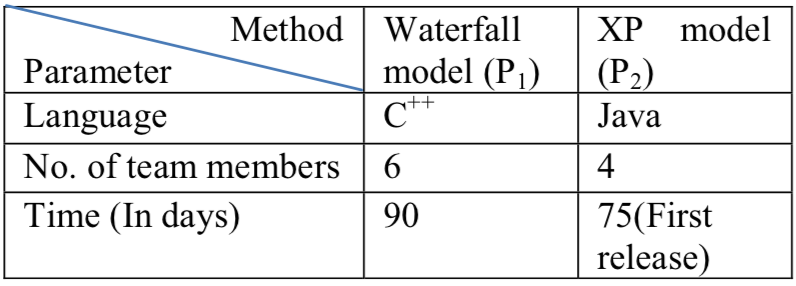
\includegraphics[scale = 0.45]{XP_vs_Waterfall.png}
 \caption[Waterfall VS XP]{Table showing a comparison in development time for both Waterfall and XP 		methodologies \citep{XPsharma2016analysis}.}
 \label{fig:XPvsWater}
\end{figure}

As the development of the project was undertaken by an individual with a limited available time as other tasks also required their own time and attention throughout the development process of this project. This made aspects of the Kanban methodology useful. One of the main benefits of the Kanban methodology is limiting the current workload on the team (or in this case, the individual) \citep{Kanban_lei2017statistical}. In this methodology only two parts of the project can be in active development at once. To start development on another part of the system one of the ``in-progress" tasks has to be completed. This helped to limit the current scope of the development, to save time, and prevent a lack of focus when balancing with other unrelated tasks.

This project had many limiting factors which dictated which parts of the development could be optimised with Software Engineering Methodologies it was important that the appropriate development system was used to deliver a working artefact on time. To do this it was not possible to use all aspects of one methodology to develop the artefact. Parts had to be taken from multiple methodologies. For example some of the more important aspects taken from the discussed methodologies were: the focus on smaller segments of the project by limiting the amount of work-in-progress items from Kanban and the fast-paced test-focused style from Extreme Programming.

\section{Tool-Sets and Machine Environments}

The tools used in any project are of the utmost importance to the completed artefact. This section will document the tools used, as well as, how, and why they were chosen for their respective roles in the project.

Arguably the most important tool used for the creation of the project is the programming language itself. In the case of this project, the language used was Python \citep{Python}. This language was used for multiple reasons. Firstly, it is compatible with many libraries which are useful to the project. This includes the OpenCV library which is vital to the project \citep{OpenCV}. Python was also used because it is able to be run on many different platforms including Mac OS, Windows and Linux-based systems. This is important to this particular artefact as the final implementation is intended to be run on a small form-factor system such as a Raspberry Pi so that it can be placed discreetly in a room and left to operate permanently. It is also a fast language to develop, not requiring as many lines of code to accomplish a task as would be required in a language such as C++. This allows for faster development which can be more effectively partnered with an agile Software Engineering Methodology.    

The OpenCV library is used in some way for all software components of the artefact which deal with video or image files. This library was chosen as it is the industry standard for computer vision libraries; it is used by ``companies like Google, Yahoo, Microsoft, Intel..." \citep{OpenCV}. Without the use of this library the project would be almost impossible to complete, especially within the given time scale for this project to be completed. The scope of the project would increase by many orders of magnitude if all of the libraries' necessary functions were required to be rewritten for this project. Using OpenCV for this purpose also has another benefit, the library is written in C++ \citep{OpenCV} which executes much faster than the Python code as it is compiled to an executable file rather than being interpreted at runtime. This allows for the program have much higher performance than if it was entirely constructed of Python code.

The software used to write the code is also very important to both the final artefact itself, and the efficiency at which it is made. The Python code for this project was written entirely within Microsoft's Visual Studio Code application for Mac OS \citep{VisualStudioCode}. This software provides a large amount of features for writing in many different languages including the Python language used for this project. The simplest of these features is the syntax highlighting which helps to make the different parts of the code easier to read. An example of the version of Visual Studio Code used is shown in Appendix A: Figure \ref{fig:VSCode}. The software can also show any errors which may be present in the code. It also features an integrated bash terminal (on Mac OS and Linux) which is useful for quickly running the program and backing up the code base using Git Version Control (this is discussed in more detail later).

Using version control and safely backing up a code base can be a vital part of any programming project. The Python code and other related files utilised the version control features of the Git version control system \citep{Git}. This system was chosen as it offers many version control features such as the ability to roll back to previous versions, clone the repository and work on the project multiple computers, and have a secure off-site backup in case of an emergency as well as other features. This was chosen over other backup solutions such as Zip-file backups or cloud services such as Dropbox for multiple reasons. Firstly, it is the industry standard method of backing up source code as it is used in the vast majority of software development situations. In one survey 88.4\% of Professional Software Developers responded that they user Git for their Version Control \citep{DeveloperSurvey}. It also offers much more resilience than other backup methods as it much less likely that the backed-up files would be deleted as it cannot be done with mouse click or short key combination like zip-file or other cloud backup could be. Even if the latest version was deleted, any other computers which have a clone of the repository and have been kept up to date would still have the code base intact. An example of the Git usage is shown in Appendix A: Figure \ref{fig:GitCommitPush} illustrating all the commands necessary for a 'git commit' and 'git push' to safely backup the entire system.

The Git Repository itself was hosted on GitHub which acted as more than just a Git Server host \citep{GitHub}, it also had some features which were useful to the project. One of the most important of these features was the issue tracker which was used to track any bugs or other issues in the software that needed to be fixed and acted as a helpful reminder. GitHub was used because it is the largest of the Git repository hosting services and most widely used by Professional Software Developers \citep{GitHubMarketShare}. A Screen shot of the GitHub Repository is shown in Appendix A: figure \ref{fig:GitRepo}.

At the beginning of the project Gantt Charts were used to plan how the available time was going to be used throughout the development process. The required features of the artefact were broken down and separated over the available time until the deadline to give each feature its time scale for completion. This original Gantt Chart is shown in Appendix A: Figure \ref{fig:OriginalGantt}. 

\chapter{Design, Development and Evaluation}

\section{Requirements Elicitation and Analysis}

The requirements for the system were initially gathered at the beginning of the development of the project from the client. The initial overall aim for the project was as follows: ``The main aim for this project is to have developed a system which can detect a human in a video using a web-cam attached to a computer, the system will be able to establish if the subject is standing or has fallen. Then, if the system detects a fall, some form of alert will be triggered".

This general aim was then abstracted into smaller, more manageable objectives to assist in making them more conceivable and accomplishable. These objectives were:

\begin{enumerate}
	\item Input the video feed from the web cam into the software so that it can be processed. The video feed should also be displayed so that the quality of the video as well as the angle of the camera can be checked.
    \item Remove the background from the video (using techniques found in the literature review) so that the silhouette of the user is left for the next stage of the program to process.
    \item Use the resultant video from the background removal to detect the position of the user’s silhouette in the video feed.
    \item Using the position of the silhouette an oval should be placed around it in the video.
    \item To determine the angle at which the subject is standing using the calculated oval (this is also using
techniques found in the literature review).
	\item Build a system for alerting a family member, carer, or friend in the event of a fall being detected by the
system.
	\item Test the system thoroughly to ensure that it can detect a fall whilst minimizing false positives.
\end{enumerate}
\noindent
The overall aim was abstracted into the objectives using research of the design of other similar systems and knowledge of how these aims could be feasibly programmed using Python. The objectives where then separated into two logical groups; Functional and Non-Functional requirements. Some more detailed requirements were also added at this stage. The functional requirements are vital to the operation of the Fall-Detection System. The Non-Functional requirements do not describe how the system operates but are still important .   

\begin{enumerate}
   \item Functional Requirements
   \begin{itemize}
   	\item Alert a family member, carer, or friend in the event of a fall being detected by the
system.
  \item Input the video feed from the web cam into the software so that it can be processed. The video feed should also be displayed so that the quality of the video as well as the angle of the camera can be checked.
      \item Remove the background from the video (using techniques found in the literature review) so that the silhouette of the user is left for the next stage of the program to process.
      \item Use the resultant video from the background removal to detect the position of the user’s silhouette in the video feed.
      \item Using the position of the silhouette an oval should be placed around it in the video.
      \item Determine the angle at which the subject is standing (using the oval from the previous requirement).
   \end{itemize}
   \item Non-Functional Requirements
    \begin{itemize}
    \item Process the video in real-time so that there is not a growing back-log of video frames which could cause the system to fill it's available memory.
	\item Test the system thoroughly to ensure that it can detect a fall whilst minimizing false positives.
    \end{itemize}
\end{enumerate}

\section{Design}

The design of the Artefact began with a simple flow diagram (This initial flow chart is shown in Figure \ref{fig:basicFlowChart}). This shows the operation of the Fall-Detection System at a high level and without much detail. The system is divided into five main stages:

\begin{enumerate}
	\item The function to import the live video stream.
    \item The function to remove the background from the current video frame leaving only the silhouette of the user.
    \item The function to detect the angle of the silhouette in the frame.
    \item The function to determine if the user has fallen using the change in the detected angle.
    \item The function to trigger an alarm or alert in the event of a detected fall.
\end{enumerate}

\begin{figure}[H]
 \centering
 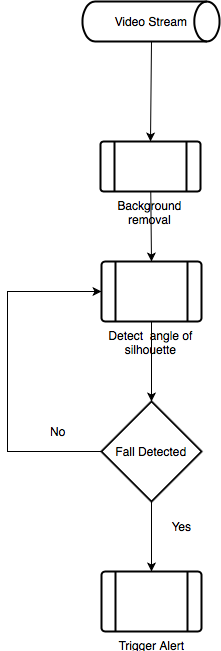
\includegraphics[scale = 0.4]{basicFlowChart.png}
 \caption[Flow Chart]{Flow Chart showing the five main sections of the Fall-Detection System.}
 \label{fig:basicFlowChart}
\end{figure}

\pagebreak
\noindent
The Flow Chart was used to design the overall architecture of the system. From the chart it was decided that the structure should be to contain four main classes which interact to perform the Fall-Detection and Alert System. The Four main classes were:
\begin{itemize}
\item backgroundRemoval()
	\begin{itemize}
	\item To remove the background from the current frame to leave the silhouette of the user.
	\end{itemize}
\item angleDetection()
	\begin{itemize}
	\item To detect the angle of the silhouette.
	\end{itemize}
\item fallDetection()
	\begin{itemize}
	\item Based on fast change in the angle detect potential falls.
	\end{itemize}
\item fallAlarm()
	\begin{itemize}
	\item Trigger an Alert in the event of a fall.
	\end{itemize}
\end{itemize}

These classes and their interactions are shown in Figure \ref{fig:UMLClassDiagram}.

\begin{figure}[H]
 \centering
 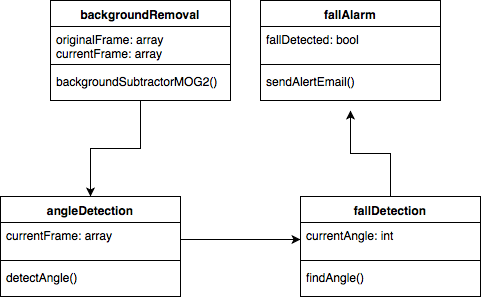
\includegraphics[scale = 0.5]{UMLClassDiagram.png}
 \caption[UML Class Diagram]{UML Class Diagram showing the four main classes of the Fall-Detection System.}
 \label{fig:UMLClassDiagram}
\end{figure}

\pagebreak

\section{Development}
The development of the system was done in an iterative manner divided into many sections or iterations. Each iteration consisted of the development of a small feature or other small part of the system, followed by testing the section which had just been implemented. The tests ensured that the new code which had been added was functioning correctly and did not interfere and cause additional bugs in the pre-existing code base.

The order in which the features were implemented in each iteration was based on the importance of the feature and whether it was required before another feature could be implemented. For example the Silhouette Angle Detection functionality had to be added before the Fall Detection functionality. The five features each to be added in their own iterations. These iterations, which collectively make up the development of the Fall-Detection System, were:

\begin{enumerate}
\item Install OpenCV library, Set up Python files and Classes, import and display video feed.
\item Effectively remove the background from the video leaving only the silhouette of the user (if the user is in the frame of the video).
\item Determine the angle of the remaining silhouette.
\item Determine if a fall has occurred.
\item In the event of a fall send an email to the specified recipient.
\end{enumerate}

\subsection{Iteration 1}

The features to be added in the first development iteration of project were relatively simple. This part the development was just concerned with creating the necessary Python files and installing the OpenCV library which was installed using Homebrew \citep{Homebrew}. The system was created across three different Python ('.py') files to keep the code base tidier and easier to maintain. These were imported using Python's 'import' functionality so that the classes contained in each file could be accessed as if they were all contained within the same file. These imports as well as the required library imports are shown in Listing \ref{PythonImports}. A screen shot showing the files created for the project is shown in Appendix B figure \ref{fig:requiredFiles}. 

\begin{listing}
\begin{minted}{Python}
import cv2, numpy as np
import angleMonitor, fallAction
\end{minted}
\caption{Python code for importing libraries and other '.py' files.}
\label{PythonImports}
\end{listing}
\noindent
The video feed can be displayed using the \textit{videoCapture()} and \textit{imshow()} functions of the OpenCV library. This is shown in Appendix B: Listing \ref{displayInputVideo}.

\subsection{Iteration 2}

The second iteration focused on removing the background from the video stream. This could be done using functions available in the OpenCV library. There were multiple background subtraction algorithms available in the library. The available algorithms were:

\begin{itemize}
  \item BackgroundSubtractorMOG
  \item BackgroundSubtractorMOG2
  \item BackgroundSubtractorGMG
\end{itemize}
\noindent
The algorithm which was used was \textit{BackgroundSubtractorMOG2} as this performed the best background subtraction and also had acceptable performance; removing the background from each frame without too much delay. This algorithm was also combined with the Morphological Operations Dilate and Erode, as well as binary thresholding to remove any noise which was left behind after the \textit{backgroundSubtractionMOG2} algorithm. The end result of the background subtraction in conjunction with the Morphological Operations is shown in Appendix B: Figure \ref{fig:backgroundSub} and a snippet of the Python code behind this is shown in Appendix B: Listing \ref{bgSubPython}.

\subsection{Iteration 3}

This development iteration focused on determining the angle of the remaining silhouette in the image. This was done using three of the available functions of OpenCV. Firstly, it needed to be determined whether the remaining non-zero pixels in the image array constituted a silhouette being present. This was done by measuring the area of the single area. The required area range which a human would occupy was found using trial and error. If an object is present in the frame inside this area range it is assumed to be a human figure. An ellipse is placed around this figure using OpenCV's \textit{fitEllipse()} function and is displayed on the video output for testing. A line is then placed through the Ellipse along its major axis. The angle of this line will then be equal to the angle at which the person is positioned in the frame. The result of this angle detection is shown in Appendix B: Figure \ref{fig:angleDetectionExample} and a code snippet of the \textit{angleDetection()} function is in Appendix B: Listing \ref{angleDetectionPython}.

\subsection{Iteration 4}
The next iteration was to find if the silhouette (if it is in the video frame) has fallen over. During this iteration the fall detection was done by measuring the angle of the major axis of the ellipse fitting around the silhouette. This is shown in Appendix C: Figure \ref{fig:fallDetected}. If the angle of the major axis falls between the range of 80\textdegree and 100\textdegree for without returning to a smaller angle this is considered to be a fall.
\begin{flushleft}
Fall-Detection system can be found at: \url{https://github.com/owenprosser/Fall-Detection}.
\end{flushleft}
\section{Testing}
The testing of the Fall-Detection System used a mixture of White-box and Black-box testing. This was done to ensure that the system was not only functioning to complete the general task correctly, but was also working efficiently. Each section of the system was tested independently following its implementation. Black-box testing was the primary testing method for the complete system as the much of the system was built upon functions included in the OpenCV library making White-box testing difficult and perhaps unnecessary.

The background subtraction was the first part of the system to be tested (it was also the first to be implemented). This was done as White-box test by watching the video output after it had been processed by the \textit{backgroundSubtraction()} function to see how effectively it was removing the background and minimising noise. An example of the output of the first iteration of the background removal is shown in Appendix C: Figure \ref{fig:bgSubNoise}. After testing and making improvements by trial-and-error the final background removal function was able to remove the background pixels of the video whilst leaving minimal noise in the image. This is shown in Appendix C: Figure \ref{fig:fallDetected}.

Once the Angle-Detection system had been implemented it was also tested. This was done in a similar manner to the testing of the background subtraction. The output of the angle detection function was displayed both on the on-screen silhouette as well as in some text at the top of the output image to make this part of the system easier to debug (shown in Appendix C: Figure \ref{fig:fallDetected}). The angle of the on-screen line was measured to make certain that the measured angle matched the one being detected by the system.

The final part of the Fall-Detection system to be implemented and tested was the fall detection. This part could be tested using both White and Black-box testing methods. Because the alerts system had not yet been created, when a fall was detected the program would output the string ``Fall Detected" to the terminal. This allowed the testing of this functionality without having to implement the full alert system (this output after a detected fall is shown in Appendix C: Figure \ref{fig:fallDetectedOutput}. Whenever the silhouette fell in the test video the output in the terminal read ``Fall Detected", showing that it was functioning correctly.

\pagebreak
\section{Operations and Maintenance}

The Fall-Detection system requires little maintenance once installed. This is because the system is designed to run without any direct interaction from the user (this was discussed previously in section 1.4) The only maintenance that could potentially be required would be to reboot the system in the event that it is not processing the live video feed in real-time and has run out of available memory storing this backlog of video frames.

\chapter{Project Conclusion}

Most of the initial aims of the project were met during the development of the Fall-Detection System. The overall objective, to be able to detect a fall when in view of the system, was met to some degree.

The System can detect falls but depending on the resolution of the video feed and the power of the hardware in which the system is running (as it is compatible with, and will run on multiple different systems) it may not run in real-time. This could cause instability, crashes, or other unexpected behaviour.

\chapter{Reflective Analysis}
Looking back across the entire development of the project I can see that there are definitely areas which can be improved the next time I am working on any project, academically or otherwise.

Firstly one of the easiest areas for improvement would be that of time management. This applies to all aspects of the project. Had the time given to develop the system been used for effectively, more features could have been added, achieving more of the initial aims and objectives. Given more time the additional features that would be added to the system would be to increase the reliability of the fall detection (using some of the methods discussed in the literature review or by performing some additional research) and to implement the alerts system so that an email can be sent to a carer or family member in the event of a fall. 

More testing of the system should have been performed to establish how well it can detect falls (this would have helped me to meet the last of my objectives). To do this I would need to record multiple videos of people falling over as I have only been using one video to develop and test the system during the creation of the artefact.

This improvement in time management could also be relevant to the methodology with which the artefact was developed. Breaking the project down into smaller sections for each iteration could have improved the time scale in which the artefact was made. The development was separated into four or five large sections each taking a week or more to complete. If I was to do this again I might break them into sections which could be completed in a few days, up to a week, to make them feel more achievable and limit the amount of time not working efficiently as I felt at times that the end of each stage was a long way off, contributing to the an increasing backlog towards the end of the project.

I also feel that I had a performed more research in the early stages of the project it would have help greatly later on in the development stages. Having a greater idea of how the system was going to run, and what the structure of it would be, would have made it much easier to develop. This research would not just have to be of academic literature but also spending more time reading the documentation for OpenCV. This could have helped me identify a better or more appropriate library function to use for part of the system for example.

I did suffer from some technical difficulties during the early stages of development which I think I will be able to avoid in the future. Firstly, I initially struggled to install the OpenCV library using bash on Mac OS. This is partly related to my previous point regarding research. Nearly all of the installation documentation I found while researching the library was aimed at Window and Linux operating systems, in part leading to installation seeming to be installed correctly whilst being inaccessible to my installed version of Python3. I the future I would be able to avoid this kind of mistake as I have learnt a lot (perhaps more than I would have without this hiccup) about the Homebrew and Pip package installers.

If the desired goal of the project was to create the most complete artefact as I could in the time frame (which was not the entire goal of this project) it would be a reasonable decision next time around to decide to develop a system in an area which I have more experience. This would help as I would have to perform less research and put more of the effort that I placed into fixing mistakes and bugs into adding more and improving the features of my artefact. I also, however, may not choose this approach in the future as I have enjoyed making something different to what have before and have learnt many valuable skills in the last year while developing the Fall-Detection system for this project.

%References
\renewcommand\bibname{References}
\addcontentsline{toc}{chapter}{References}
\bibliography{references.bib}
\pagebreak
\clearpage

%Appendices
\appendix
\section{Appendices}
\subsection{Appendix A}

\begin{figure}[h]
 \centering
 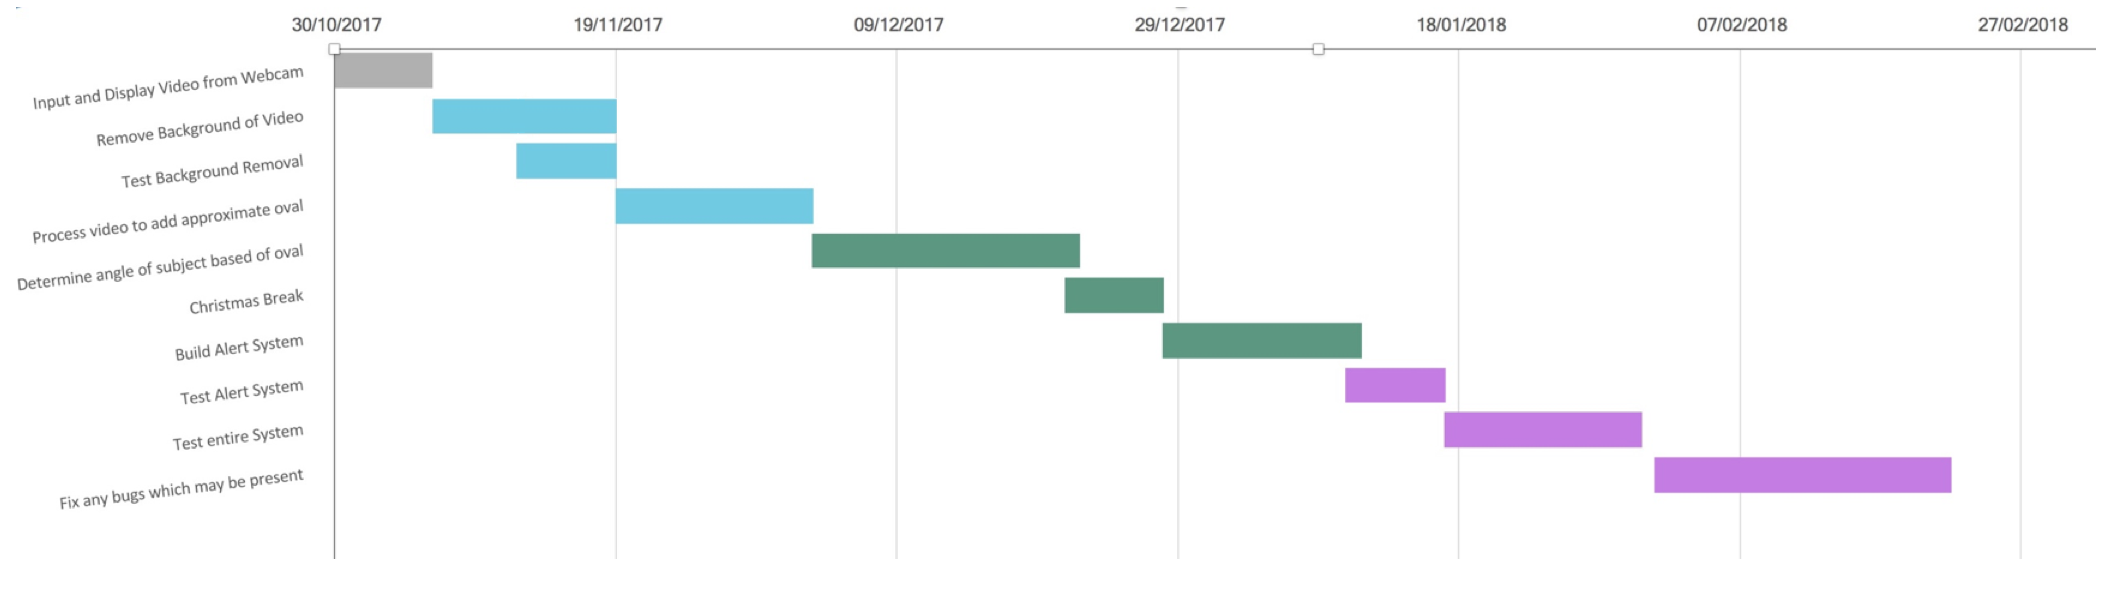
\includegraphics[scale = 0.33]{Original_gantt_chart.png}
 \caption[Original Gantt Chart]{Original Gantt Chart for the planned project timescale.}
 \label{fig:OriginalGantt}
\end{figure}

\begin{figure}[h]
 \centering
 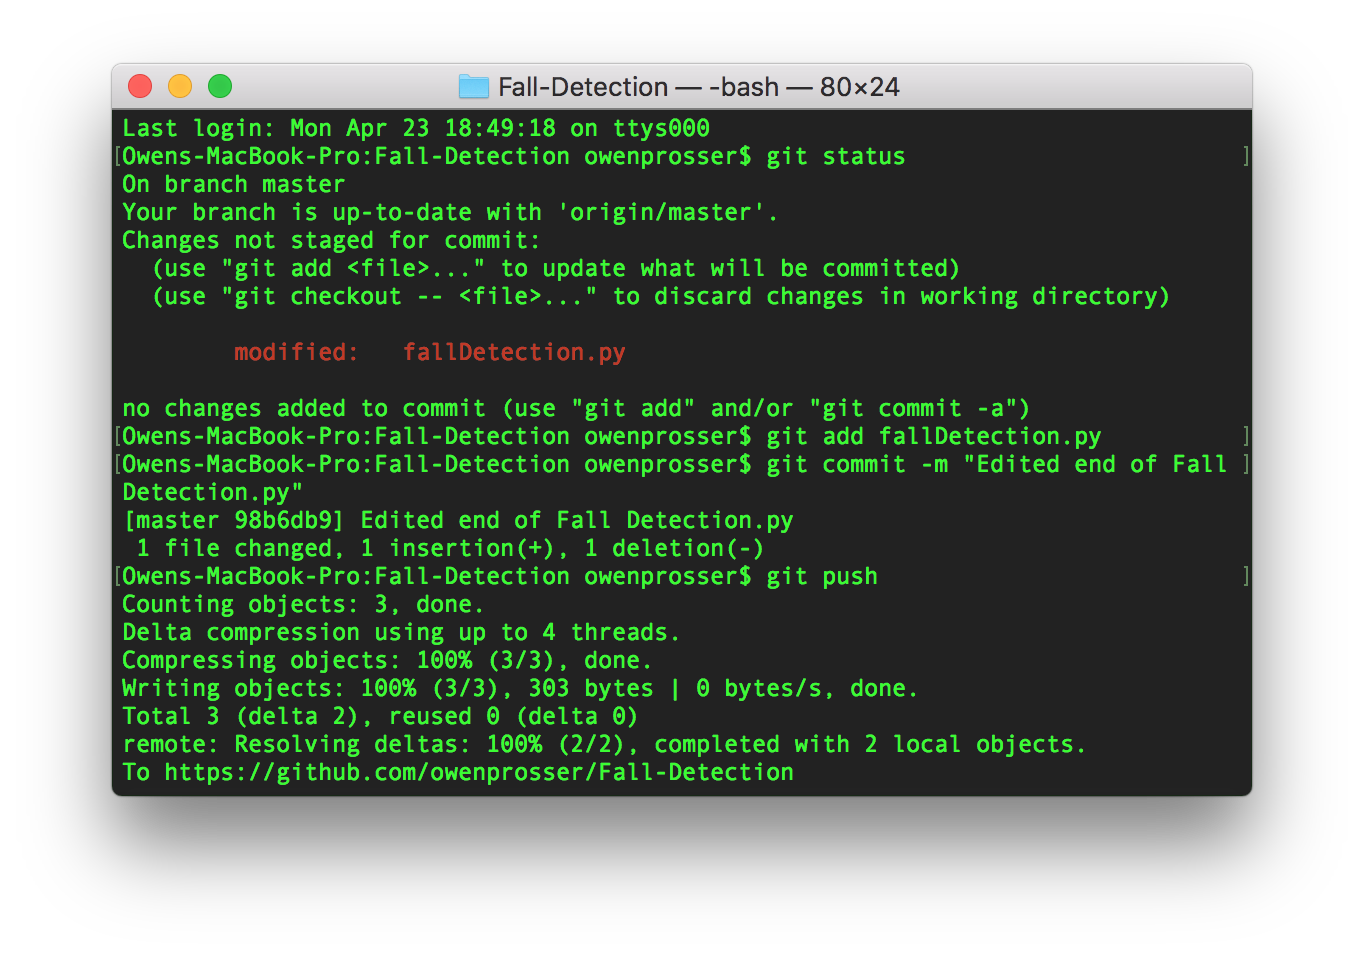
\includegraphics[scale = 0.55]{gitpush.png}
 \caption{Example of git commit and push commands.}
 \label{fig:GitCommitPush}
\end{figure}

\begin{figure}[H]
 \centering
 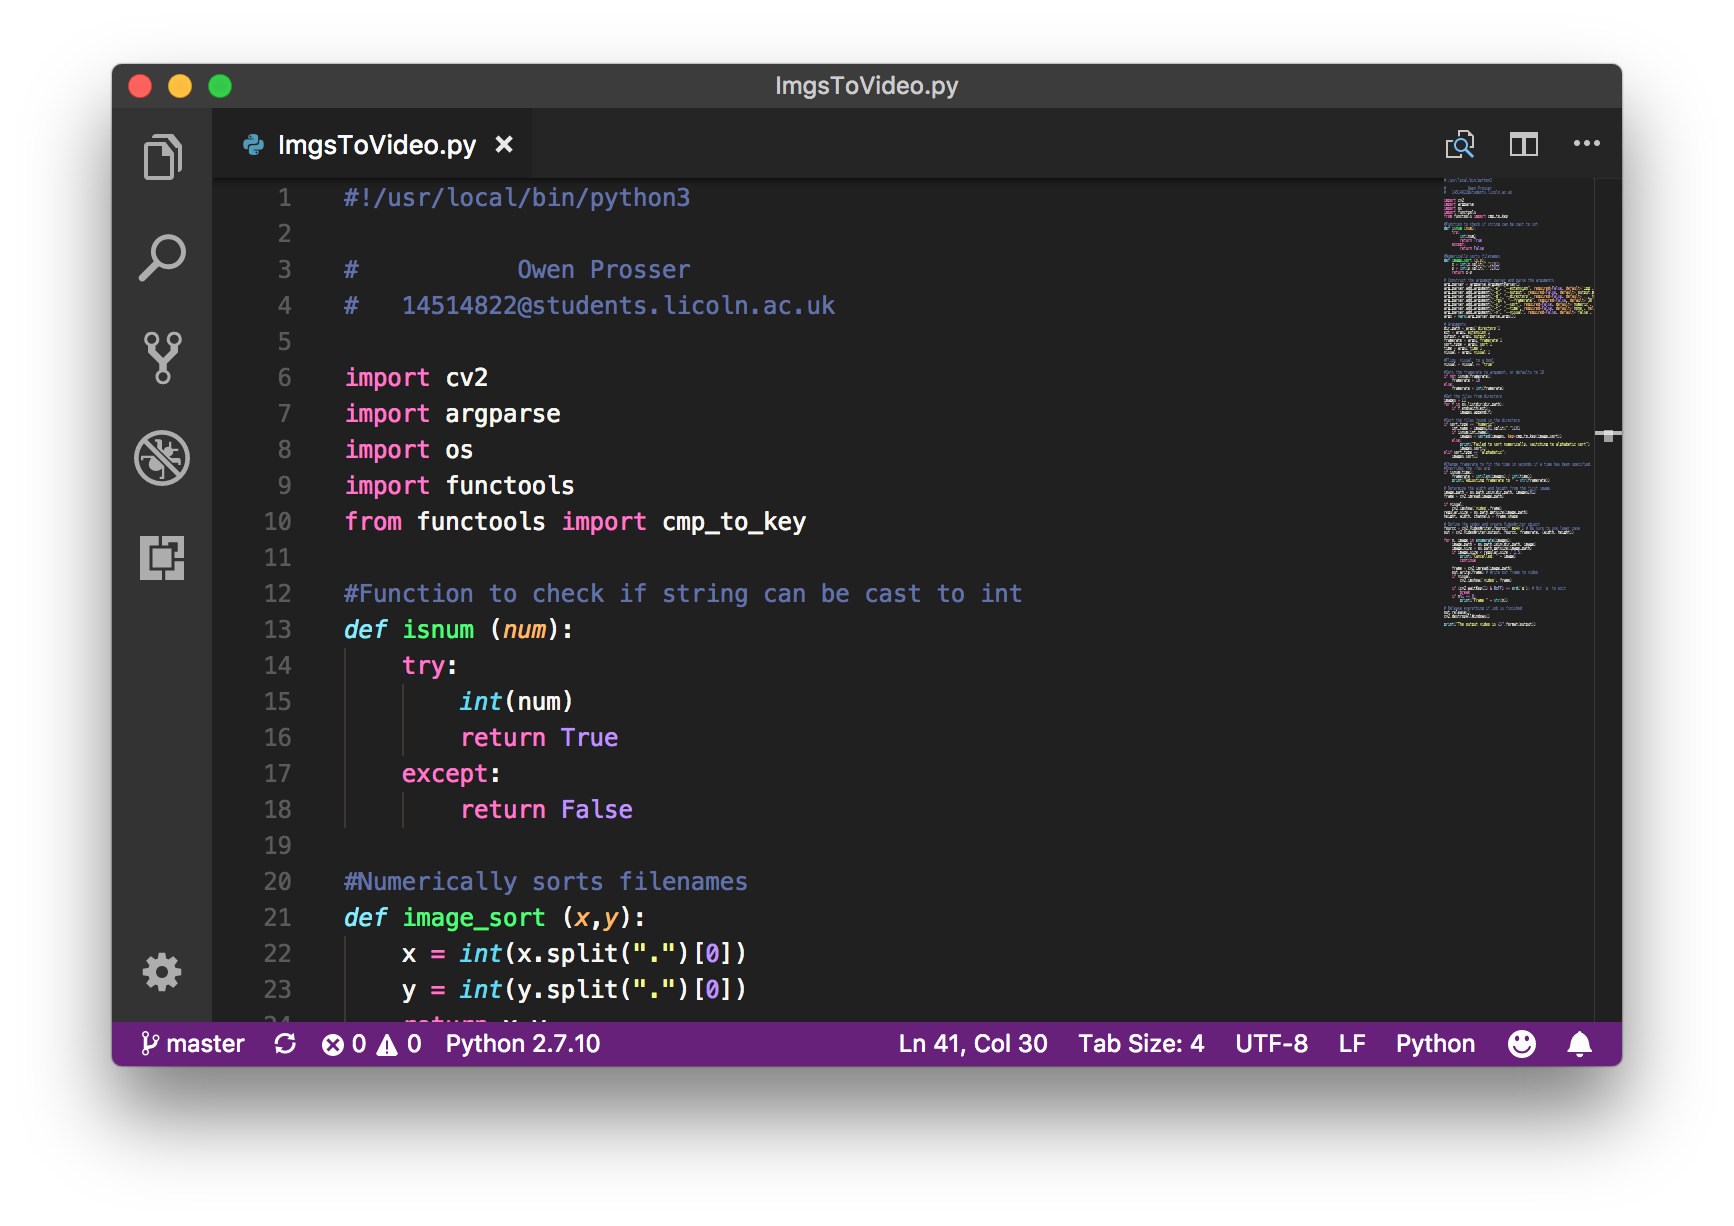
\includegraphics[scale = 0.4]{VSCode.png}
 \caption[Syntax Highlighted Code]{Example of Python code in Visual Studio Code with Syntax Highlighting}
 \label{fig:VSCode}
\end{figure}

\begin{figure}[H]
 \centering
 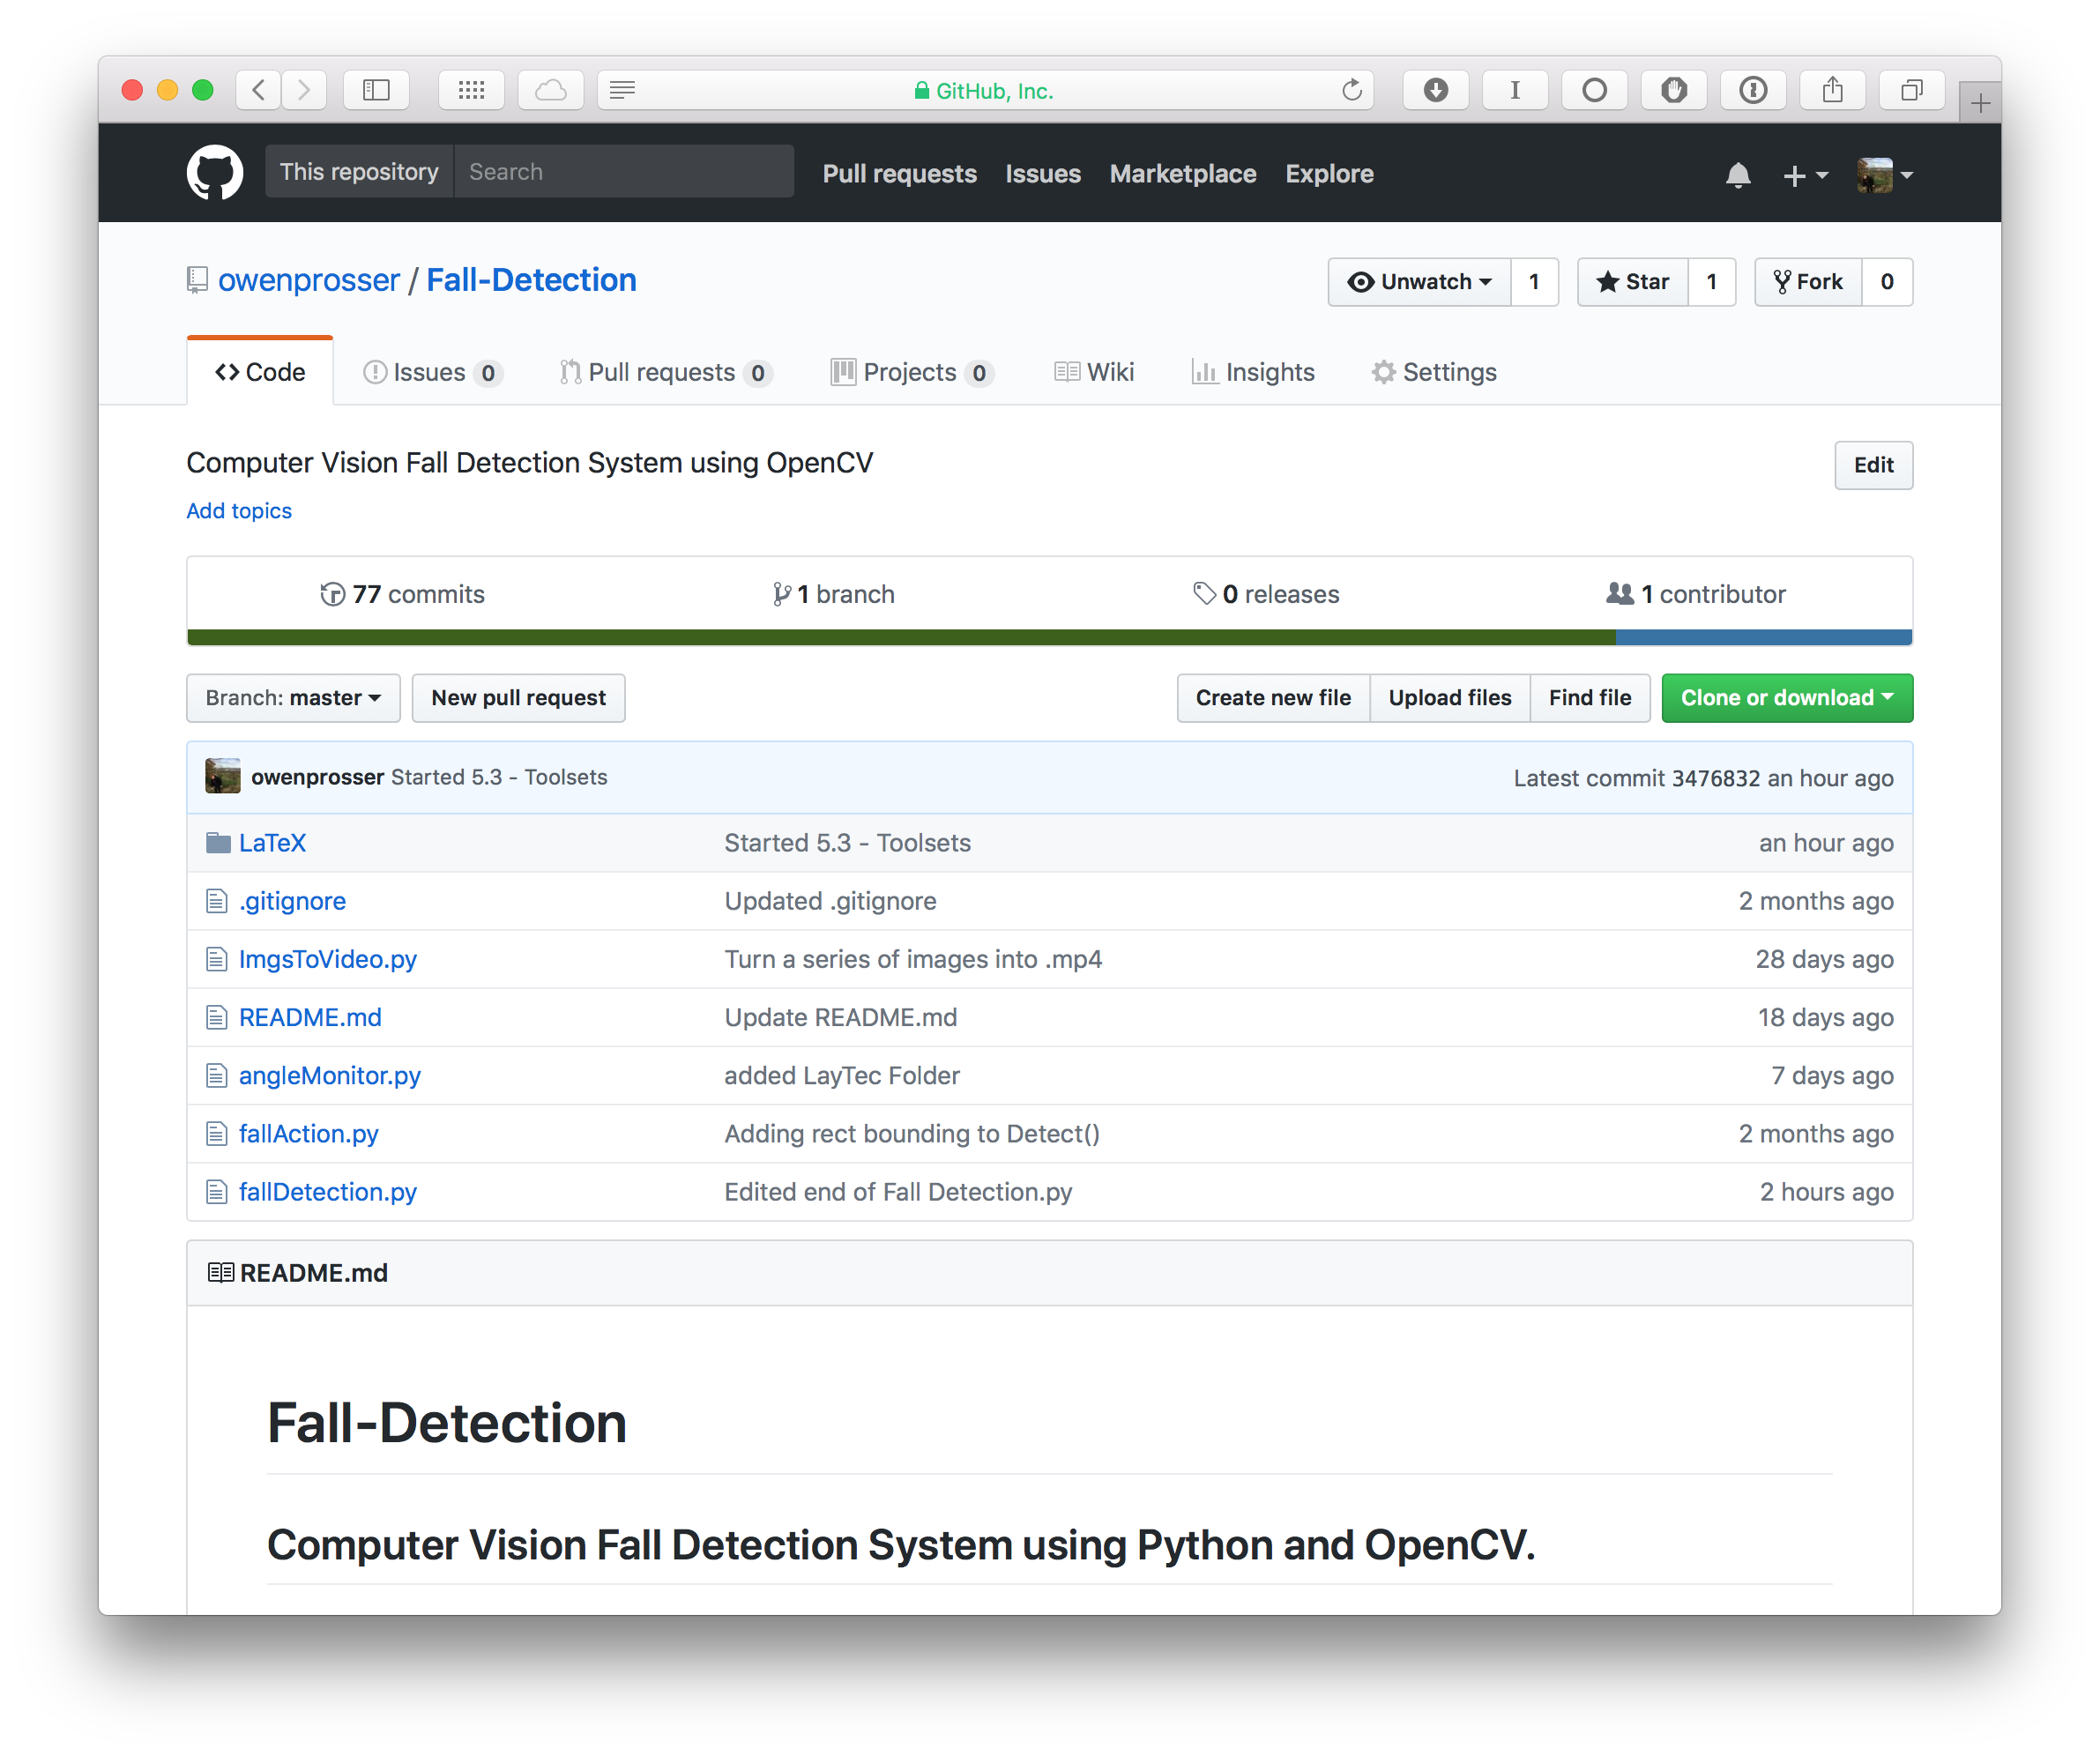
\includegraphics[scale = 0.14]{GitRepo.png}
 \caption[Git Repository]{Screen shot of the Git Repository Hosted on http://github.com.}
 \label{fig:GitRepo}
\end{figure}

\subsection{Appendix B}

\begin{figure}[H]
 \centering
 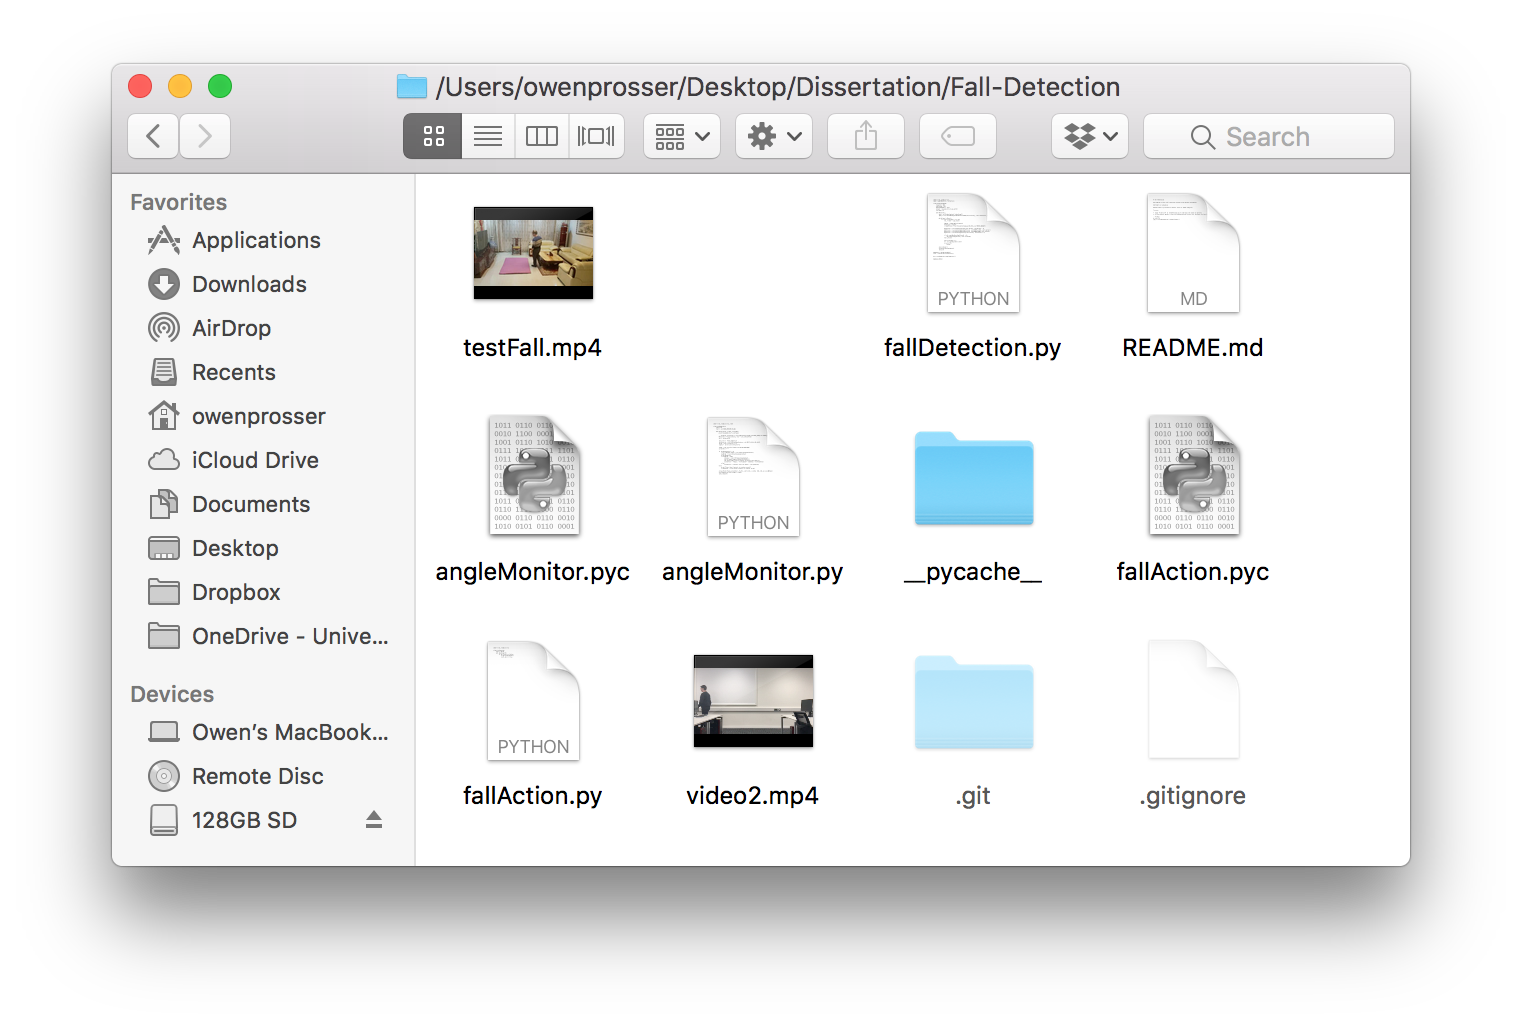
\includegraphics[scale = 0.5]{requiredFiles.png}
 \caption[Necessary Files]{'.py' and other files needed for the system.}
 \label{fig:requiredFiles}
\end{figure}

\begin{listing}
\begin{minted}{Python}
while(cap != None):
  cap = cv2.VideoCapture(0)
  if (self.curFrame % 1 == 0):
    ret, frame = cap.read()
    cv2.imshow("Current Frame", frame)
    self.curFrame += 1
    k = cv2.waitKey(30) & 0xff
  if k == 27:
  	break
cap.release()
cv2.destroyAllWindows()
return 0
\end{minted}
\caption{Python code snippet to show live webcam feed using OpenCV.}
\label{displayInputVideo}
\end{listing}

\begin{figure}[H]
 \centering
 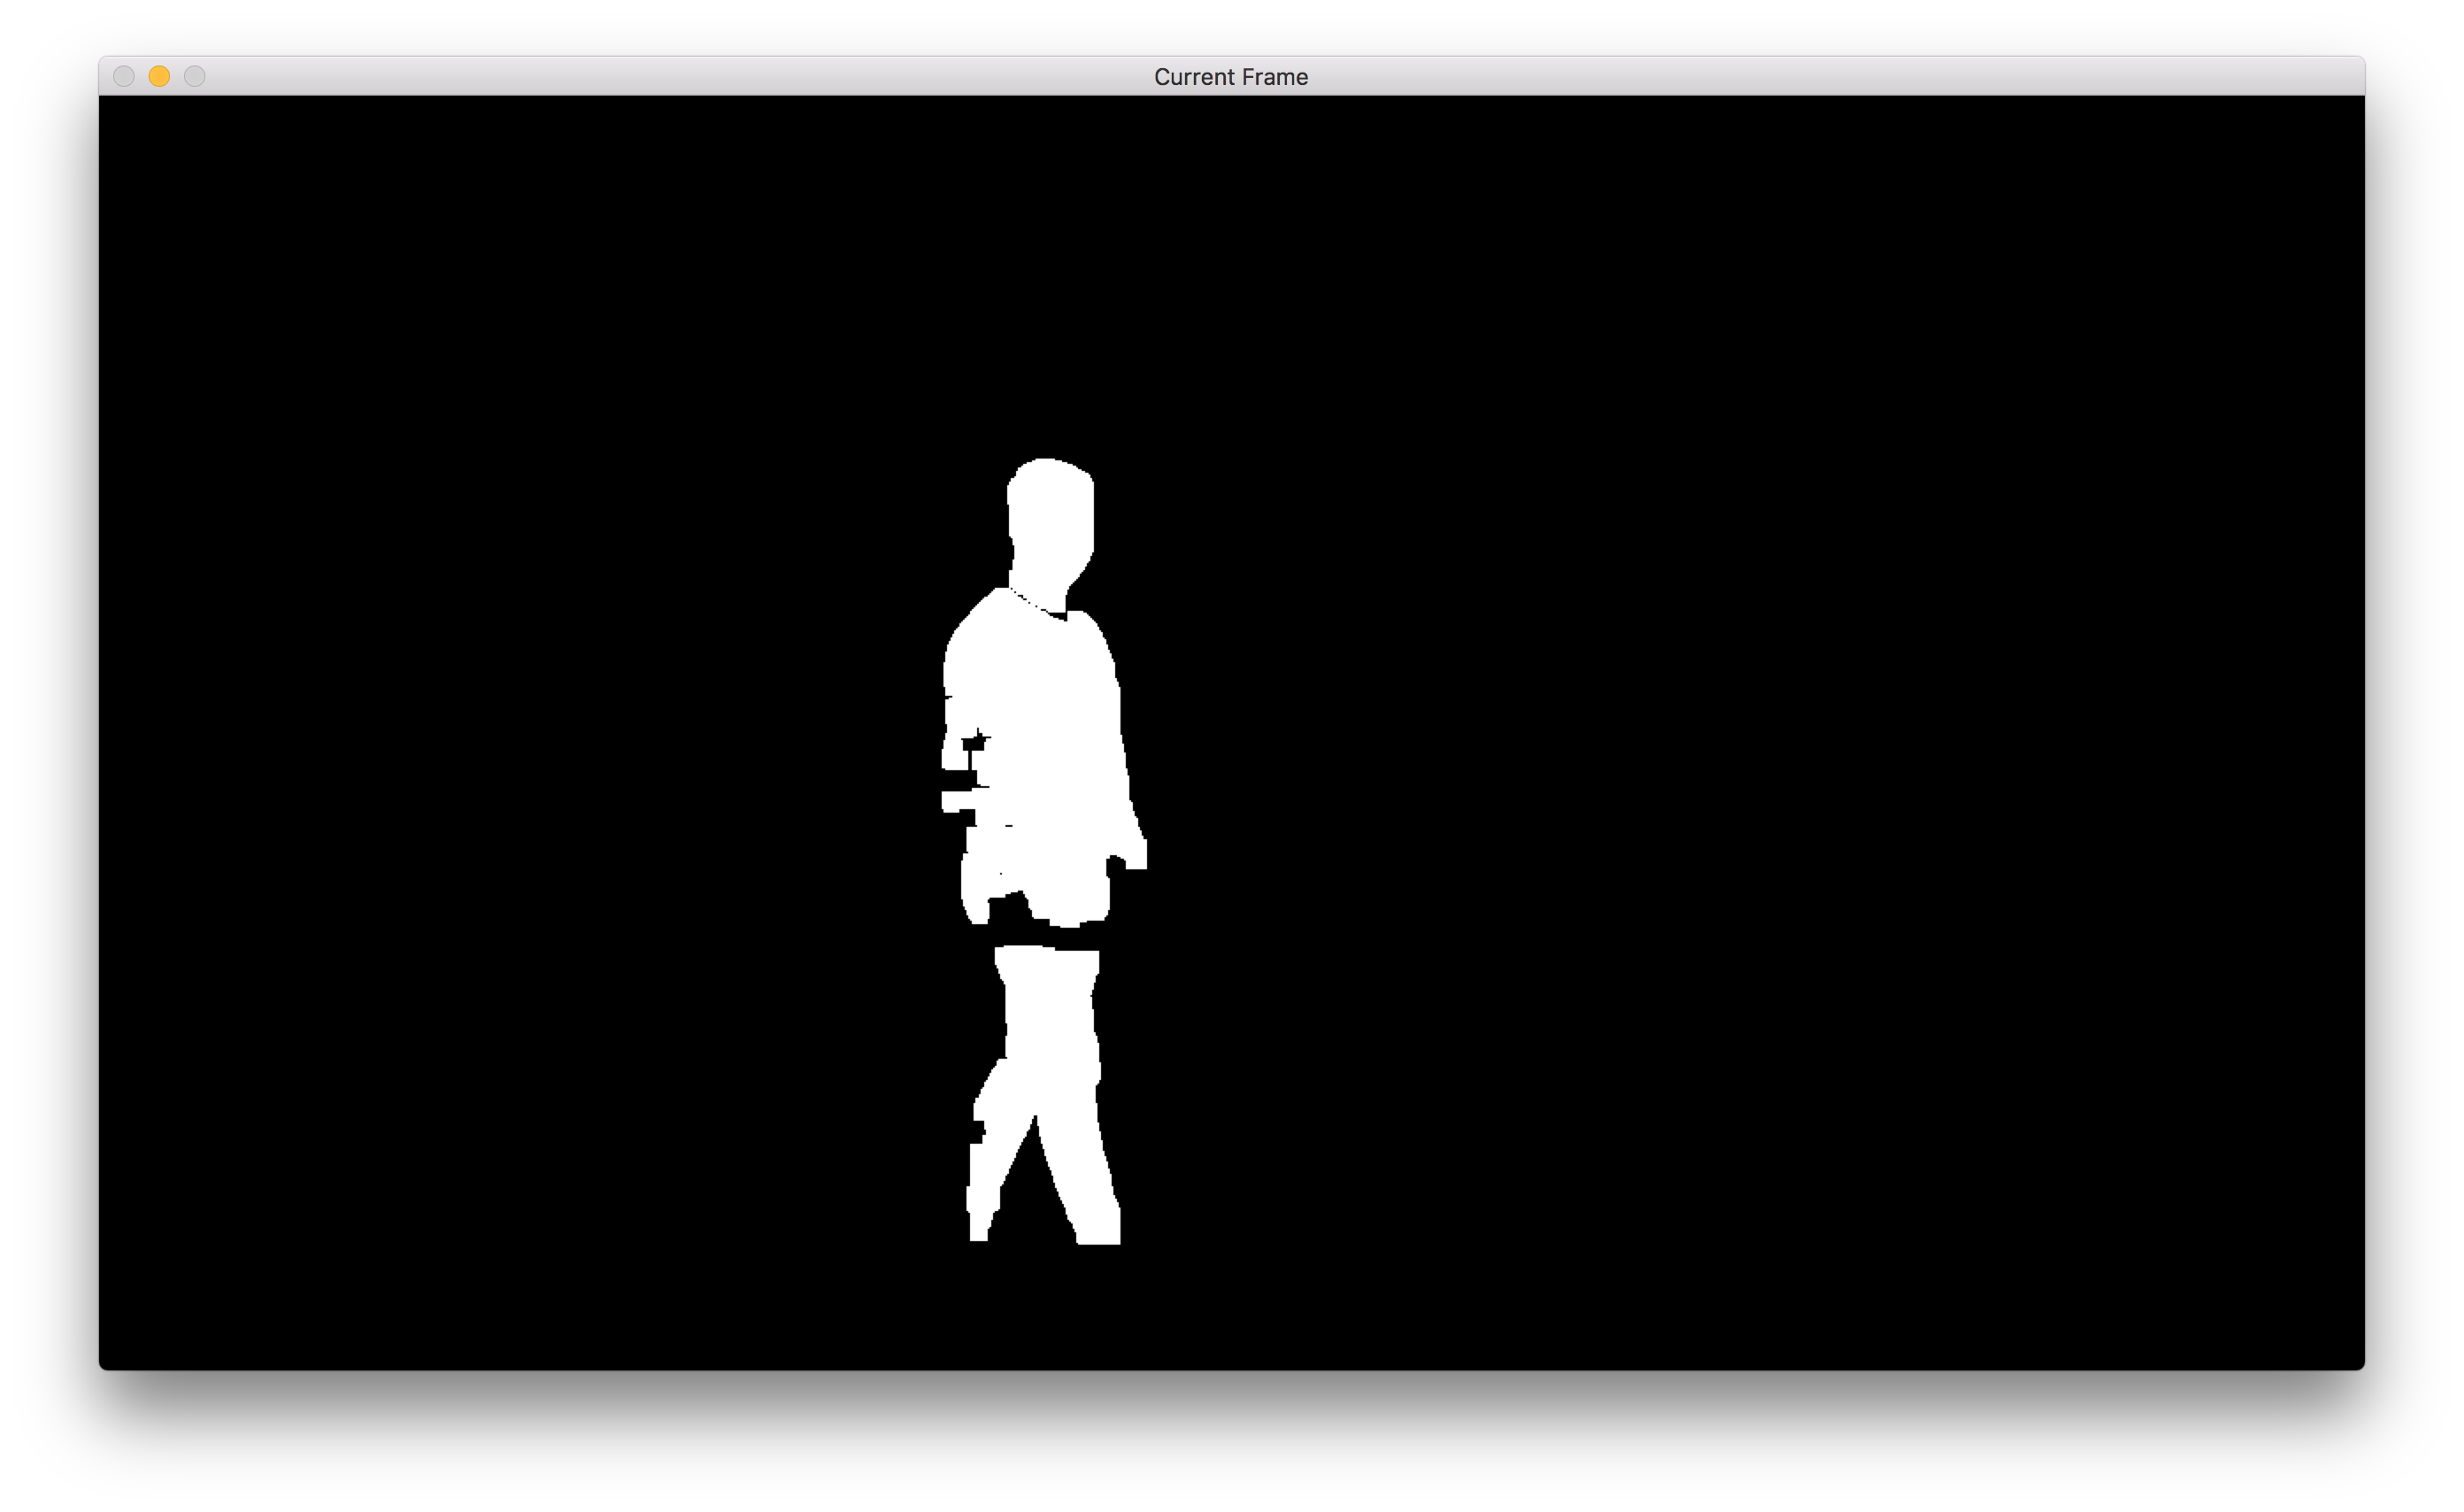
\includegraphics[scale = 0.22]{bgSubExample.png}
 \caption[Background Subtraction]{Screen shot showing the effectiveness of the backgroudSubtractorMOG2() algorithm with Morphological Operations.}
 \label{fig:backgroundSub}
\end{figure}

\begin{listing}
\begin{minted}{Python}
def MOG(self):
  cap = cv2.VideoCapture('video2.mp4')
  fgbg = cv2.createBackgroundSubtractorMOG2(self.history, 
  self.varThresh ,self.detectShadows)
  while(cap != None):
    if (self.curFrame % 1 == 0):
      ret, frame = cap.read()
      fgmask = fgbg.apply(frame,0)
      bgrThresh = fgmask
      _, bgrThresh = cv2.threshold(fgmask,250,255,cv2.THRESH_BINARY)
      bgrThresh = cv2.erode(bgrThresh,self.kernel, iterations = 1)
      bgrThresh = cv2.morphologyEx(bgrThresh, cv2.MORPH_CLOSE, self.kernel)
      bgrThresh = cv2.morphologyEx(bgrThresh, cv2.MORPH_OPEN, self.kernel)
      bgrThresh = cv2.dilate(bgrThresh,self.kernel, iterations = 1)
      if cv2.countNonZero(bgrThresh) > 0:
      	det.Detect(bgrThresh, self.curFrame)
      self.curFrame += 1
      k = cv2.waitKey(30) & 0xff
      if k == 27:
      	break
cap.release()
cv2.destroyAllWindows()
return 0
\end{minted}
\caption{Python for Background Subtraction and Morphological Operations.}
\label{bgSubPython}
\end{listing}

\begin{figure}[H]
 \centering
 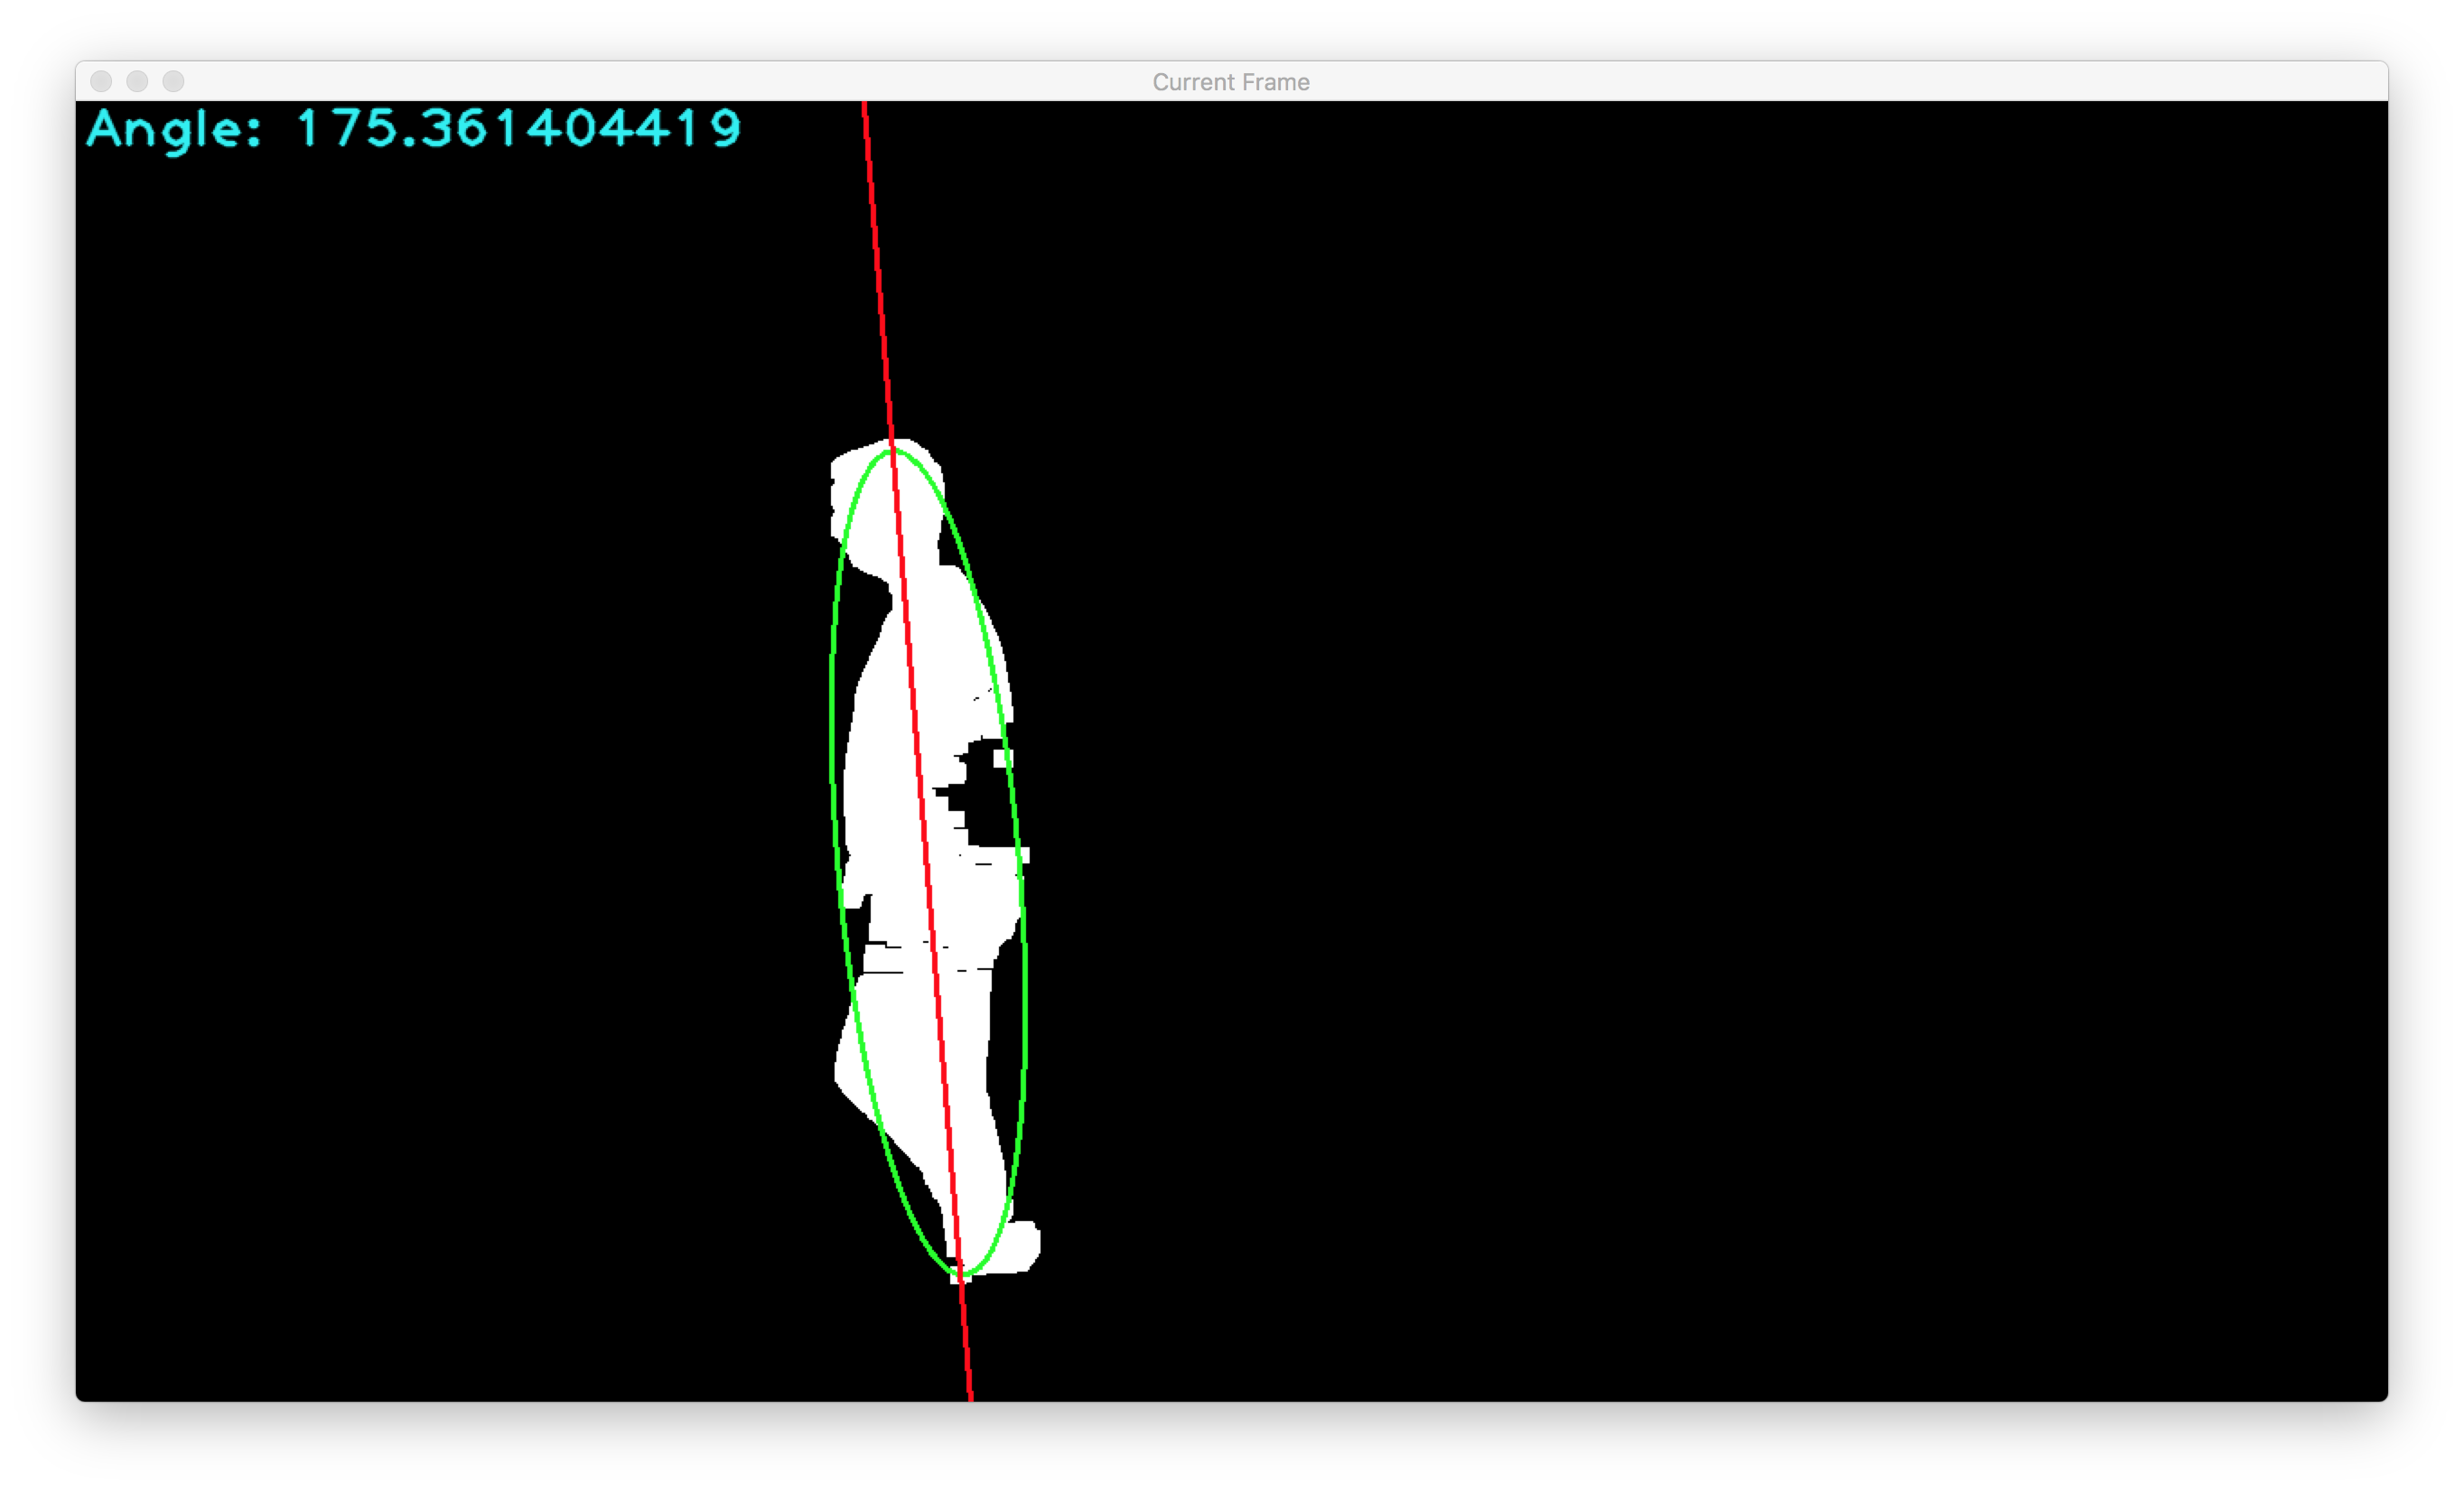
\includegraphics[scale = 0.22]{angleExample.png}
 \caption[Angle Detection]{Screen shot showing the output from the \textit{angleDetection()} function.}
 \label{fig:angleDetectionExample}
\end{figure}

\begin{listing}
\begin{minted}{Python}
def Detect(self, frame, curFrame):
  _, contours, hierarchy = cv2.findContours(frame,cv2.RETR_TREE,
  cv2.CHAIN_APPROX_SIMPLE)
  maxContour = max(contours, key = cv2.contourArea)
  cnt = contours[0]

  rows,cols = frame.shape[:2]
  [vx,vy,x,y] = cv2.fitLine(maxContour, cv2.DIST_L2,0,0.01,0.01)
  lefty = int((-x*vy/vx) + y)
  righty = int(((cols-x)*vy/vx)+y)

  frame = cv2.cvtColor(frame,cv2.COLOR_GRAY2RGB)
  screenText = ""

  if len(maxContour) > 4:
    (x,y),(MA,ma),angle = cv2.fitEllipse(maxContour)
    maxArea = cv2.contourArea(maxContour)
    print(maxArea)
    if maxArea > 100:
      ellipse = cv2.fitEllipse(maxContour)
      cv2.ellipse(frame,ellipse,(0,255,0),2)
      cv2.line(frame,(cols-1,righty),(0,lefty),(0,0,255),2)
      screenText = 'Angle: '+str(angle)
\end{minted}
\caption{Python code for angle detection.}
\label{angleDetectionPython}
\end{listing}

\subsection{Appendix C}

\begin{figure}[H]
 \centering
 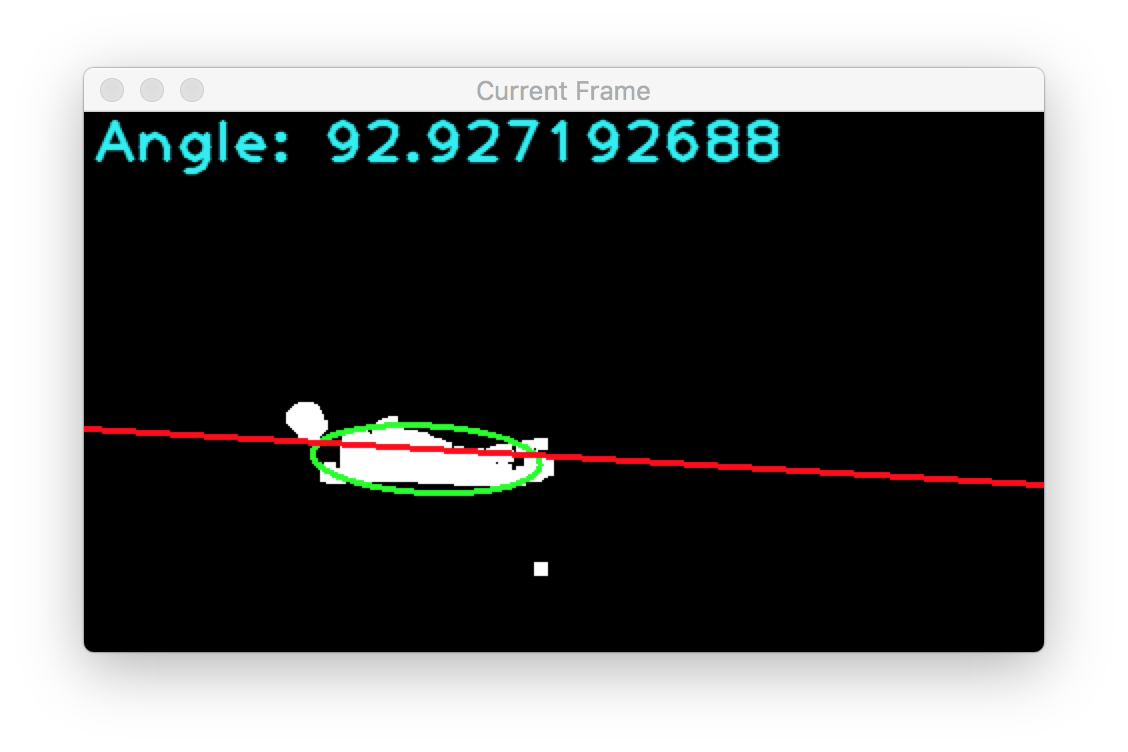
\includegraphics[scale = 0.6]{fallDetected.png}
 \caption[Fall Detection]{Screen shot showing the output during the detection of a fall.}
 \label{fig:fallDetected}
\end{figure}

\begin{figure}[H]
 \centering
 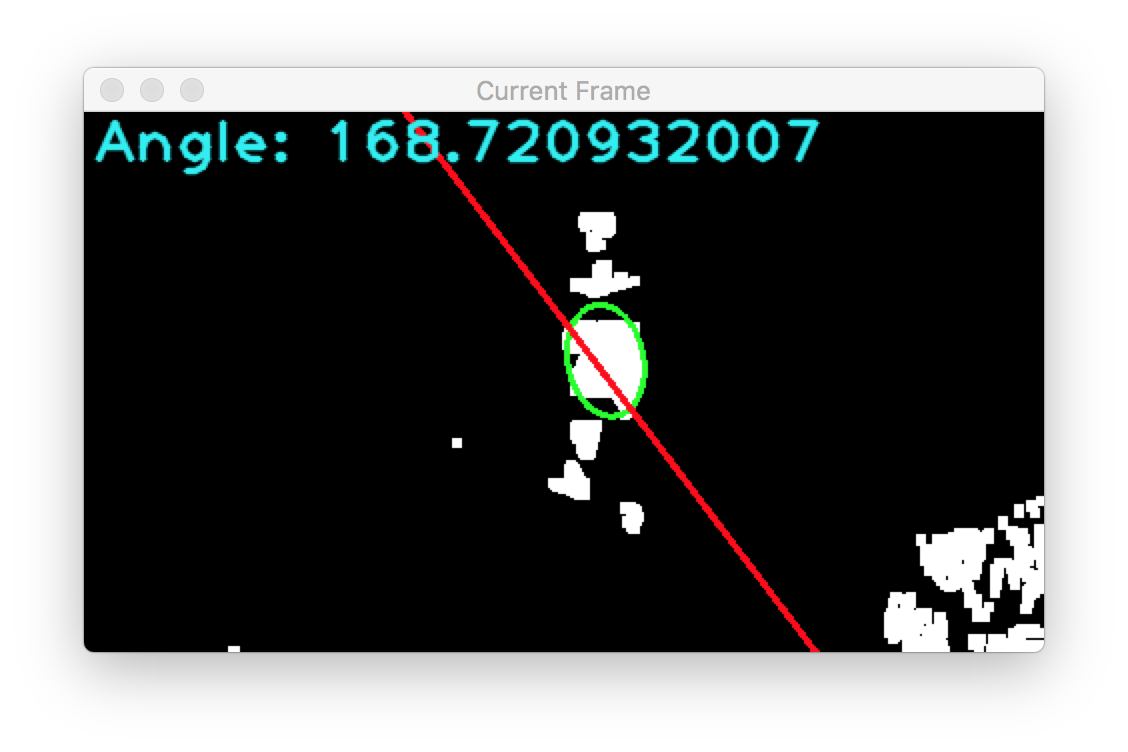
\includegraphics[scale = 0.6]{bgSubNoise.png}
 \caption[Original Background Subtraction]{Screen shot showing the remaining noise after processing by an early version of the background subtraction function.}
 \label{fig:bgSubNoise}
\end{figure}

\begin{figure}[H]
 \centering
 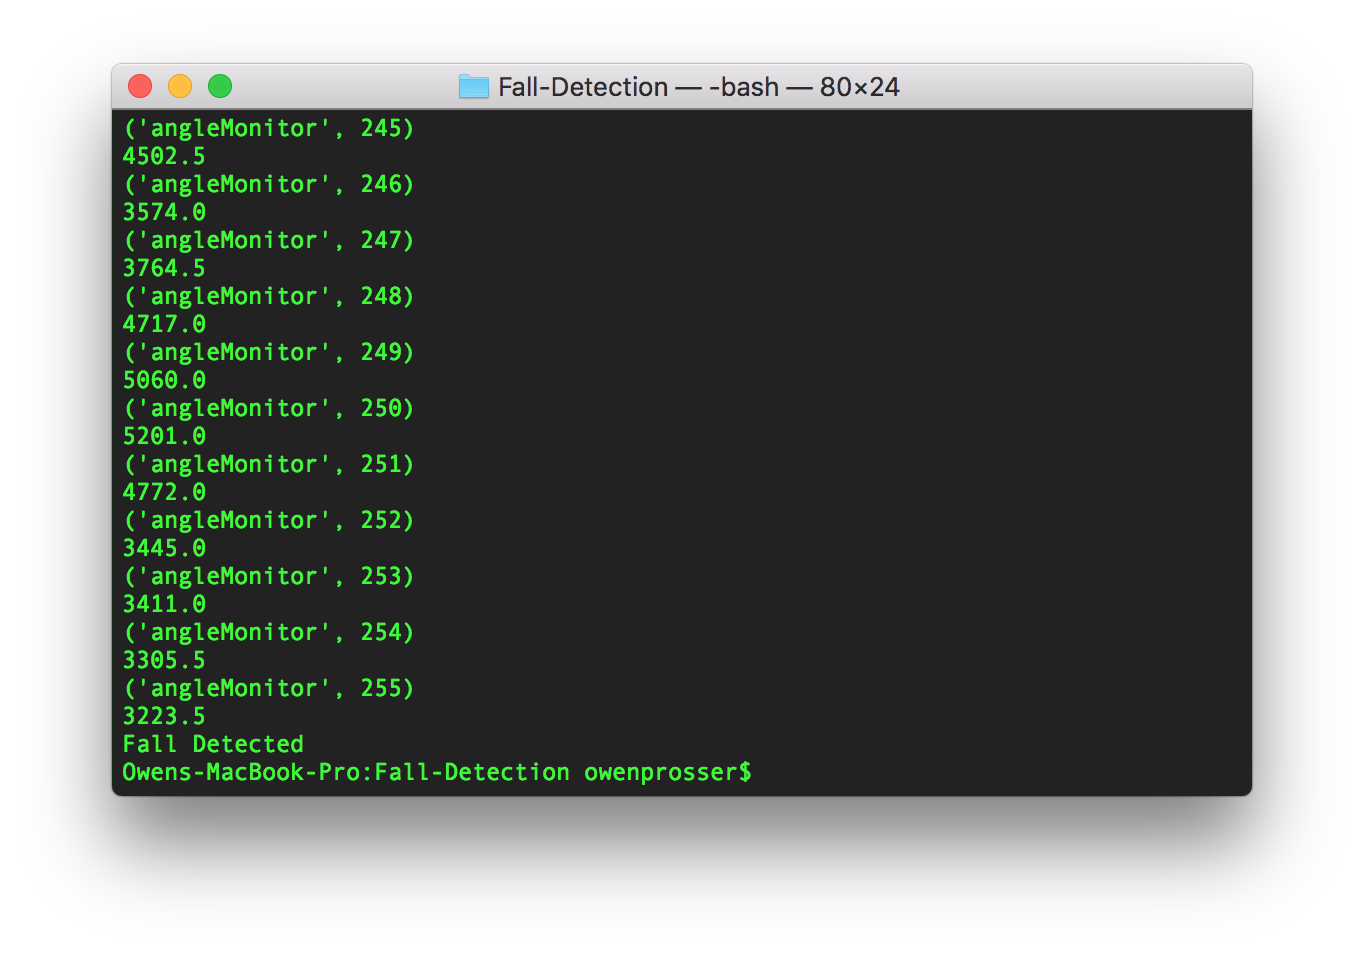
\includegraphics[scale = 0.5]{fallDetectedOutput.png}
 \caption[Bash Terminal Output]{Screen shot showing the output to the terminal in the event of detecting a fall.}
 \label{fig:fallDetectedOutput}
\end{figure}

\end{document}